The Sun produces its energy through nuclear fusion reactions occurring in its core. Gravitational compression of the Sun's mass generates a central region with densities exceeding $150\,\text{g}/\text{cm}^3$ and temperatures near $15 \times 10^6\,\text{K}$. Under these conditions, nuclear interactions become energetically accessible, allowing hydrogen nuclei to fuse into helium and releasing binding energy in the process.

In the simplest view, fusion proceeds through direct collisions of hydrogen nuclei. At core temperatures of order $15 \times 10^6\,\text{K}$, protons possess sufficient thermal kinetic energy to approach closely enough for the strong nuclear force to bind them. Through a sequence of interactions known as the proton–proton chain, four protons are ultimately transformed into a helium nucleus. 

Each fusion event in the Sun's core releases a small amount of energy — approximately $26.7\,\text{MeV}$ per helium nucleus formed. However, the Sun generates a total power output of roughly $3.8 \times 10^{26}\,\text{W}$, which requires converting mass to energy at an enormous rate. By Einstein's relation $E = mc^2$, this luminosity implies a mass loss of about $4.3 \times 10^9\,\text{kg}$ per second. That is, the Sun converts over four million tonnes of mass into energy every second, almost entirely from the fusion of hydrogen into helium.

This mass loss is not directly visible but manifests as outward radiation pressure. Deep within the core, energy liberated by fusion builds up pressure that counteracts gravitational collapse. The resulting hydrostatic equilibrium maintains the Sun's overall structure: every second, the immense weight of the Sun's outer layers is balanced by pressure generated from fusing approximately $6 \times 10^{11}$ kilograms of hydrogen into helium. The Sun's long-term stability emerges from this balance — fusion sustains the outward force needed to resist the crushing pull of its own mass.

The energy generated in the core does not escape immediately. Photons produced during fusion undergo radiative diffusion, scattering thousands of times off electrons and nuclei as they migrate outward. In the outer layers, convective transport becomes dominant, with rising and sinking plasma transporting energy. After this complex migration, energy is finally emitted from the photosphere as sunlight, spanning a broad electromagnetic spectrum.

However, the conservation of energy alone is insufficient to guarantee physical consistency in nuclear reactions. In addition to energy, momentum and electric charge must be conserved exactly at every interaction vertex. Quantum field theories of particle interactions also impose another conserved quantity: lepton number. Leptons — a class of particles including electrons, neutrinos, and their antiparticles — must be created or destroyed in such a way that the total lepton number remains unchanged in any fundamental process.

The proton–proton chain, which powers the Sun, involves changes in particle types that require mechanisms beyond the electromagnetic and strong forces. In particular, the weak nuclear force is necessary to enable the conversion of protons into neutrons while preserving all conservation laws. Without the weak force, the fusion of hydrogen into helium could not proceed.

A key reaction illustrating these requirements is the first step of the chain:
\[
\text{p} + \text{p} \;\to\; \text{d} + e^+ + \nu_e,
\]

where $\text{p}$ denotes a proton, $\text{d}$ a deuteron (a bound state of one proton and one neutron), $e^+$ a positron, and $\nu_e$ an electron neutrino. In this reaction, one proton transforms into a neutron through a weak interaction. To conserve electric charge, a positron — the antimatter counterpart of the electron — is emitted. To conserve lepton number, an electron neutrino is emitted simultaneously. 

In the lepton number accounting, electrons and neutrinos are assigned a lepton number of $+1$, while positrons and antineutrinos carry a lepton number of $-1$. Before the reaction, the system has zero net lepton number; after the reaction, the positron ($-1$) and neutrino ($+1$) balance each other, maintaining overall neutrality. The emission of the neutrino is therefore a necessity for the reaction to be consistent with the fundamental symmetries of particle physics.

Although neutrinos possess extremely small mass and interact only via the weak force, they carry away a significant fraction of the reaction's energy and linear momentum. Unlike photons, which scatter thousands of times before reaching the solar surface, neutrinos traverse the Sun's dense interior with minimal interaction and escape into space almost immediately. Neutrinos produced in the Sun's core reach Earth in about 8 minutes, providing a direct and real-time probe of nuclear processes occurring deep inside the Sun.

The detection of solar neutrinos has been crucial for confirming theoretical models of stellar energy generation. Measurements not only validate the dominance of the proton–proton chain but also reveal minor contributions from alternative fusion pathways, such as the carbon–nitrogen–oxygen (CNO) cycle.

Quantum mechanics introduces behaviors absent in classical physics. One of the most fundamental is tunneling: the ability of a particle to penetrate and traverse a potential barrier even when its total energy is insufficient to overcome it. 

Classically, a particle with energy less than the height of a potential barrier would be fully reflected, with zero probability of passage. Motion would be confined to regions where the total energy exceeds the potential energy. In quantum mechanics, however, particles are described by continuous wavefunctions governed by the Schrödinger equation. Even in classically forbidden regions, the wavefunction persists, decaying exponentially rather than vanishing abruptly.

When a quantum particle encounters a barrier higher than its energy, its wavefunction inside the barrier takes the form of a decaying exponential. If the barrier has finite width, there exists a nonzero probability that the particle will appear beyond the barrier — a phenomenon known as quantum tunneling. The probability of tunneling depends sensitively on the height and width of the barrier, with taller or wider barriers leading to exponentially smaller transmission probabilities.

Mathematically, for a particle of energy $E$ encountering a barrier of height $V_0 > E$, the tunneling probability $P$ scales approximately as
\[
P \sim e^{-2\gamma d},
\]
where $d$ is the barrier width and
\[
\gamma = \frac{\sqrt{2m(V_0 - E)}}{\hbar},
\]
with $m$ the particle mass and $\hbar$ the reduced Planck constant. The existence of tunneling thus follows directly from the mathematical structure of quantum mechanics, requiring no special assumptions beyond the continuity of the wavefunction and the validity of the Schrödinger equation.


\begin{figure}[H]
\centering
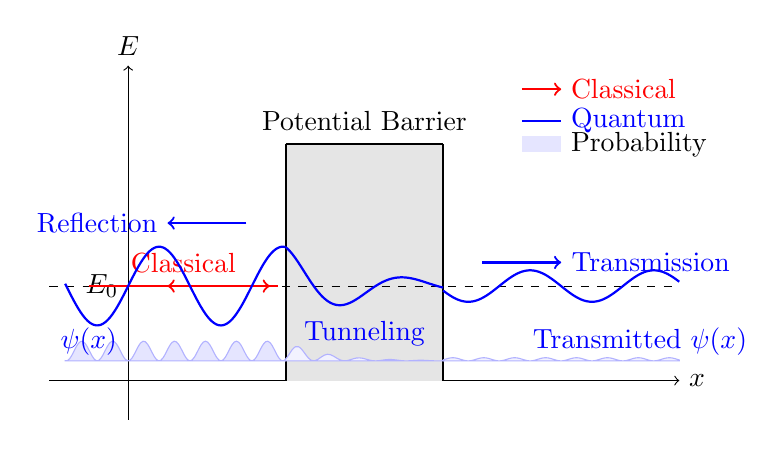
\begin{tikzpicture}[scale=1.0]
    % Axis with better labels
    \draw[->] (-1,0) -- (7,0) node[right] {$x$};
    \draw[->] (0,-0.5) -- (0,4) node[above] {$E$};
    
    % Potential Barrier (smoother edges)
    \fill[gray!20] (2,0) rectangle (4,3);
    \draw[thick] (2,0) -- (2,3);
    \draw[thick] (4,3) -- (4,0);
    \draw[thick] (2,3) -- (4,3);
    \node at (3,3.3) {Potential Barrier};
    
    % Energy Level with better labeling
    \draw[dashed] (-1,1.2) -- (7,1.2);
    \node[left] at (0,1.2) {$E_0$};
    
    % Classical Particle Trajectory
    \draw[->, thick, red] (-0.5,1.2) -- (1.8,1.2);
    \draw[->, thick, red] (1.9,1.2) -- (0.5,1.2);
    \node[red] at (0.7,1.5) {Classical};
    
    % Quantum Wavefunction (improved visualization)
    % Incident wave
    \draw[blue, thick, domain=-0.8:2, samples=100, smooth] plot(\x,{0.5*sin(deg(4*\x))+1.2});
    
    % Exponentially decaying wave in barrier
    \draw[blue, thick, domain=2:4, samples=50, smooth] plot(\x,{0.5*exp(-1*(\x-2))*sin(deg(4*\x))+1.2});
    
    % Transmitted wave with reduced amplitude
    \draw[blue, thick, domain=4:7, samples=100, smooth] plot(\x,{0.2*sin(deg(4*\x))+1.2});
    
    % Probability density for incident wave
    \draw[blue!30, domain=-0.8:2, samples=100, smooth, fill=blue!10] plot(\x,{0.25*sin(deg(8*\x))*sin(deg(8*\x))+0.25}) -- (2,0.25) -- (-0.8,0.25) -- cycle;
    
    % Probability density in barrier (decaying)
    \draw[blue!30, domain=2:4, samples=50, smooth, fill=blue!5] plot(\x,{0.25*exp(-2*(\x-2))*sin(deg(8*\x))*sin(deg(8*\x))+0.25}) -- (4,0.25) -- (2,0.25) -- cycle;
    
    % Probability density for transmitted wave (smaller)
    \draw[blue!30, domain=4:7, samples=100, smooth, fill=blue!5] plot(\x,{0.04*sin(deg(8*\x))*sin(deg(8*\x))+0.25}) -- (7,0.25) -- (4,0.25) -- cycle;
    
    % Labels and annotations - repositioned to avoid overlap
    \node[blue] at (-0.5,0.5) {$\psi(x)$};
    \node[blue] at (3,0.6) {Tunneling};
    \node[blue] at (6.5,0.5) {Transmitted $\psi(x)$};
    
    % Reflection and transmission arrows - adjusted positions
    \draw[->, blue, thick] (1.5,2.0) -- (0.5,2.0) node[left] {Reflection};
    \draw[->, blue, thick] (4.5,1.5) -- (5.5,1.5) node[right] {Transmission};
    
    % Legend - moved to top right corner with better spacing
    \draw[thick, red, ->] (5.0,3.7) -- (5.5,3.7);
    \node[red, right] at (5.5,3.7) {Classical};
    \draw[thick, blue] (5.0,3.3) -- (5.5,3.3);
    \node[blue, right] at (5.5,3.3) {Quantum};
    \fill[blue!10] (5.0,2.9) rectangle (5.5,3.1);
    \node[right] at (5.5,3.0) {Probability};
\end{tikzpicture}
\caption{Quantum tunneling allows a particle to penetrate and cross a potential barrier even when its total energy ($E_0$) is less than the barrier height. Classically, the particle would be fully reflected, but quantum mechanics permits a non-zero probability of transmission through the barrier. The wavefunction $\psi(x)$ decays exponentially inside the barrier but emerges with reduced amplitude on the other side.}
\end{figure}

In the solar core, the fusion of protons faces a major obstacle: the Coulomb barrier arising from electrostatic repulsion. The potential energy associated with two protons at close approach is approximately $1\,\text{MeV}$, whereas the typical thermal kinetic energy at $15 \times 10^6\,\text{K}$ is about $1\,\text{keV}$. Classically, the probability of overcoming the barrier would be vanishingly small, and fusion would be effectively impossible.

Despite this, fusion proceeds because quantum tunneling allows protons to penetrate the Coulomb barrier with nonzero probability. Rather than requiring kinetic energies comparable to the barrier height, quantum mechanics enables fusion at energies far below the classical threshold. The proton wavefunctions extend into and through the classically forbidden region, resulting in occasional barrier penetration and subsequent nuclear fusion.

The probability of tunneling through the Coulomb barrier is quantified by the Gamow factor. This factor arises from solving the Schrödinger equation for two charged particles and introduces an exponential suppression depending on the product of the charges, the reduced mass of the system, and the relative kinetic energy. Specifically, the tunneling probability scales as
\[
P \sim \exp\left( -\frac{b}{\sqrt{E}} \right),
\]
where \( b \) is a constant depending on fundamental parameters such as the fine-structure constant and the masses and charges involved.

At stellar core temperatures, the Gamow factor dominates the fusion reaction rate. Although tunneling is rare on a per-collision basis, the immense number of available protons ensures that sufficient fusion events occur to sustain the Sun's energy output. The exponential sensitivity of the tunneling probability to temperature means that small variations in core temperature result in large changes in the fusion rate.

Stars like the Sun shine because of nuclear fusion, a process that converts mass into energy in their cores. But under classical physics, the conditions inside the Sun — although extreme by terrestrial standards — would be insufficient to allow protons to overcome their mutual electrostatic repulsion and collide. The average thermal energy at core temperatures of $1.5 \times 10^7\,\text{K}$ is only about $1\,\text{keV}$, far below the $1\,\text{MeV}$ scale required to surmount the Coulomb barrier. Without an additional mechanism, fusion rates would be negligible, and the Sun would be incapable of generating the energy required to support itself against gravity.

The energy production rate in the Sun is set by the interaction between thermal motion and quantum tunneling. At core temperatures of $1.5 \times 10^7\,\text{K}$, the average kinetic energy of protons remains far below the Coulomb barrier. Tunneling enables rare collisions to result in fusion, and the total rate of such events determines the outward energy flux. This rate must match the gravitational compression exerted by the Sun's mass. If it were too low, contraction would increase the central temperature until equilibrium was restored; if it were too high, expansion would reduce the reaction rate. The equilibrium point defines a narrow band of possible core conditions that are dynamically stable over long timescales.

This regulatory mechanism underlies the existence of the main sequence: the phase in stellar evolution during which hydrogen fusion occurs in the core at a steady rate. A star remains on the main sequence as long as the supply of hydrogen in the central region is sufficient to sustain the fusion rate required for equilibrium. The lifetime of this phase depends on the star's mass, which sets both the compression rate and the temperature needed to counteract it. For the Sun, this balance produces a stable configuration lasting approximately $10^{10}$ years.

The observed constancy of the Sun's luminosity results from a dynamically stable interaction between gravity, fusion kinetics, and quantum penetration probabilities. These parameters jointly determine the rate at which mass is converted to energy and transported outward. Over time, this energy supports the weight of the overlying layers without abrupt expansion or collapse.

The apparent simplicity of the Sun's structure conceals the extreme improbability of its processes. Each reaction in the core depends on a tunneling event through a high-energy barrier. The Sun radiates steadily only because the number of collisions is vast enough to produce a reliable average. On longer timescales, the gradual depletion of hydrogen shifts the core structure, altering the tunneling profile and initiating the next evolutionary stage. The duration and character of stellar equilibrium thus reflect specific quantum constraints built into the energy landscape of nuclear matter.

Neutrinos represent one of the most intriguing particles produced by solar fusion. These ghostly particles carry the fundamental properties of an electron — including its half-integer spin and status as a fermion — but lack electric charge entirely. In the Standard Model of particle physics, fermions are governed by the Pauli exclusion principle and contribute to the conservation of fermion number in all interactions. When a proton transforms into a neutron during the initial step of the proton-proton chain, the process must preserve not only energy and momentum, but also fermion number.

The weak nuclear force enables this transformation by converting one of the proton's up quarks into a down quark, effectively changing the proton's identity to that of a neutron. However, this conversion alone would violate fermion number conservation. To restore balance, the reaction simultaneously creates a positron and an electron neutrino. The positron, being the antimatter counterpart of an electron, carries a fermion number of $-1$, while the neutrino carries $+1$. This pairing ensures that the total fermion number remains unchanged throughout the process.

The Sun produces neutrinos at a staggering rate. Every second, approximately $2 \times 10^{38}$ neutrinos escape from the solar core, representing roughly $2\%$ of the total energy released by fusion. These particles possess extraordinarily small interaction cross-sections — about $10^{-44}\,\text{cm}^2$ for typical solar neutrino energies — making them effectively invisible to ordinary matter. While photons generated in the core require thousands of years to diffuse through the Sun's dense interior, neutrinos escape almost instantaneously, traveling from the core to Earth in just over 8 minutes.

This property makes solar neutrinos a direct and real-time probe of nuclear processes occurring deep within the Sun. Every neutrino detected on Earth was produced moments earlier in a fusion reaction at the solar core. By measuring the flux and energy spectrum of these particles, scientists can test theoretical models of stellar energy generation with unprecedented precision.

However, when physicists first attempted to detect solar neutrinos in the 1960s, they encountered a profound puzzle. Raymond Davis Jr.'s pioneering experiment, conducted in the Homestake Mine in South Dakota, used a tank containing 400,000 liters of perchloroethylene to capture neutrinos through the reaction:
\[
\nu_e + \text{Cl}^{37} \;\to\; e^- + \text{Ar}^{37}.
\]

The Homestake detector measured only about one-third of the neutrino flux predicted by standard solar models. This deficit, known as the solar neutrino problem, persisted for over three decades despite increasingly sophisticated experiments and refinements to stellar theory.

The resolution came through the discovery of neutrino oscillations — a quantum mechanical phenomenon in which neutrinos spontaneously transform between different types, or "flavors," as they propagate through space. The Standard Model recognizes three distinct neutrino flavors: electron neutrinos ($\nu_e$), muon neutrinos ($\nu_\mu$), and tau neutrinos ($\nu_\tau$). Solar fusion produces exclusively electron neutrinos, but if these particles oscillate into other flavors during their journey to Earth, early detectors — which were sensitive only to electron neutrinos — would register an apparent deficit.

The breakthrough came from experiments capable of detecting all neutrino flavors simultaneously. The Sudbury Neutrino Observatory (SNO), located 2 kilometers underground in Ontario, Canada, used heavy water ($\text{D}_2\text{O}$) to measure both the total neutrino flux and the flux of electron neutrinos specifically. SNO's results, announced in 2001, confirmed that the total neutrino flux matched theoretical predictions exactly, but that approximately two-thirds of the electron neutrinos had oscillated into other flavors by the time they reached Earth.

Neutrino oscillations can only occur if neutrinos possess nonzero mass. In the original formulation of the Standard Model, neutrinos were assumed to be massless, like photons. The discovery of oscillations therefore constituted evidence for physics beyond the Standard Model and demonstrated that neutrinos, while extraordinarily light, do have finite masses. Current measurements indicate that neutrino masses are less than a few tenths of an electron volt — over a million times smaller than the electron mass — but definitively nonzero.

This discovery resolved the solar neutrino problem and provided crucial validation of both solar fusion theory and quantum field theory. The flux of neutrinos reaching Earth precisely matches the rate predicted by models of nuclear burning in the solar core. Moreover, the phenomenon of oscillations has opened new avenues in fundamental physics, including investigations of CP violation in the lepton sector and potential implications for cosmology and the matter-antimatter asymmetry of the universe.

While neutrinos provide a direct probe of nuclear processes in the solar core, other observational techniques allow scientists to study the Sun's interior structure and dynamics. Helioseismology — the study of solar oscillations — enables detailed mapping of conditions throughout the solar interior, from the photosphere down to the core.

The Sun undergoes continuous acoustic oscillations driven by convective motions in its outer layers. These oscillations generate pressure waves that propagate through the solar interior, much like seismic waves travel through Earth's interior during earthquakes. The frequencies, amplitudes, and spatial patterns of these oscillations depend sensitively on the temperature, density, and composition profiles within the Sun.

Solar oscillations are observed as periodic Doppler shifts in absorption lines from the photosphere. The Global Oscillation Network Group (GONG) and space-based missions such as the Solar and Heliospheric Observatory (SOHO) continuously monitor these oscillations with extraordinary precision. Millions of distinct oscillation modes have been identified, each characterized by specific radial and angular patterns of motion.

By analyzing the frequencies of different oscillation modes, helioseismologists can infer the internal structure of the Sun through a process analogous to medical imaging. Just as seismic tomography reveals Earth's internal structure from earthquake data, solar oscillations provide a three-dimensional map of temperature, density, and rotation rate as functions of depth and latitude within the Sun.

Helioseismological measurements have confirmed key predictions of stellar models with remarkable accuracy. The inferred temperature profile matches theoretical expectations to within $0.1\%$ throughout most of the solar interior. The depth of the convective zone — the region where energy transport occurs primarily through convective motion rather than radiation — has been measured to be $0.287$ solar radii from the surface, in excellent agreement with theoretical models.

Perhaps most importantly, helioseismology has validated the density and temperature profiles used to predict solar neutrino production. The central temperature inferred from oscillation data is $15.7 \pm 0.1$ million K, confirming the conditions required for the proton-proton chain to operate at the observed rate. This independent confirmation of core conditions strengthens confidence in both stellar evolution theory and the understanding of nuclear processes governing solar energy generation.


\begin{SideNotePage}{
  \textbf{Top: Solar Fusion and Quantum Tunneling:} This diagram illustrates the \textbf{proton-proton (pp) chain}, the dominant fusion process in the Sun's core, where hydrogen nuclei (protons) fuse into helium, releasing energy. Here's the breakdown of the stages shown:
  \vspace{1em}
  \textbf{Stage 1: Proton-Proton Fusion} — Two \textbf{protons (red)} fuse to form: A \textbf{deuteron} (one proton + one neutron — shown here as red + blue), A \textbf{positron} (green), and A \textbf{neutrino} (ν). This happens twice independently. \textbf{Reaction:} $p + p \rightarrow \text{D} + e^+ + \nu_e$
  
  \vspace{1em}
  \textbf{Stage 2: Deuteron-Proton Fusion} — The deuteron (p+n) fuses with another \textbf{proton (red)} to form: \textbf{Helium-3 (two protons, one neutron — 2 red + 1 blue)} A \textbf{gamma ray} (γ), indicating energy release. This also occurs in parallel twice. \textbf{Reaction:} $\text{D} + p \rightarrow \text{He-3} + \gamma$

  \vspace{1em}
  \textbf{Stage 3: Helium-3 Fusion} — Two \textbf{helium-3 nuclei} collide, forming: One \textbf{helium-4 nucleus} (2 protons + 2 neutrons — 2 red + 2 blue), Two free \textbf{protons} (red), released back to the plasma. \textbf{Reaction:} $\text{He-3} + \text{He-3} \rightarrow \text{He-4} + 2p$
  \vspace{1em}
  \textbf{Net Result} — The chain converts \textbf{4 protons into 1 helium-4 nucleus}, with: Energy carried by \textbf{gamma rays}, \textbf{neutrinos}, and \textbf{kinetic energy} of the particles, Two protons recycled. This chain is responsible for the Sun's energy production, light, and the solar neutrinos we detect on Earth.
  \vspace{3em}
  \textbf{Bottom: Quantum Tunneling} enables this entire process by allowing particles to skip energy barriers. The barrier doesn't stop the particle completely but rather dampens the probability wave without zeroing it. This quantum mechanical effect permits fusion to occur at the Sun's core temperature (15 million K), where classical physics would predict negligible fusion rates due to insufficient thermal energy to overcome the Coulomb barrier between protons.
}{10_SolarFusionQuantumTunneling/UNPOPSCI - solar fusion + quantum tunneling .pdf}
\end{SideNotePage}